
\section{Uniform Bundle and Item Pricing}

In this section, we present a brief discussion for worst-case guarantees on how well uniform bundle pricing and item pricing can approximate the 
optimal subadditive and monotone bundle pricing. Figure~\ref{fig:summary} summarizes the upper and lower bounds that are either known,
or we obtain in this paper.


\begin{figure}[t]
	\scalebox{.95}{
		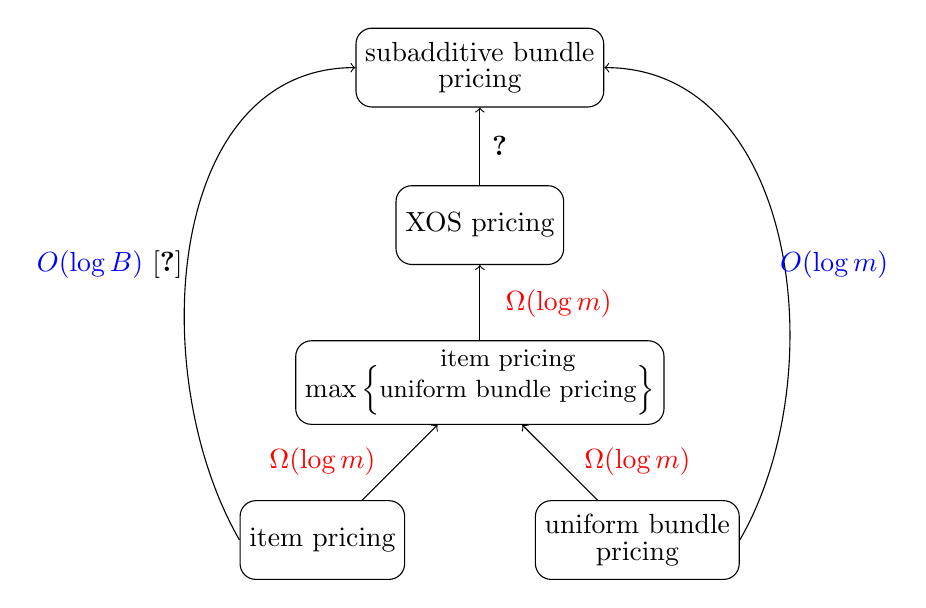
\begin{tikzpicture}
		\tikzset{recstyle/.style={rectangle, draw, minimum width=7mm, minimum height=10mm,rounded corners=.2cm}}
		
		%\node[recstyle] (rectsum) at (0,1.5) {$\sum_{e \in \mE} v_e$};
		\node[recstyle] (rectbundle) at (0,0.5) {\shortstack{subadditive bundle \\ pricing}};
		\node[recstyle] (rectxos)  at (0,-1.5) {XOS pricing};
		\node[recstyle] (rectmax) at (0,-3.5) {$\max \Big\{  \shortstack{\small item pricing \\ \small uniform bundle pricing} \Big\}$};
		\node[recstyle] (rectitem) at (-2,-5.5) {item pricing};
		\node[recstyle] (rectubundle)  at (2,-5.5) {\shortstack{uniform bundle \\ pricing}};
		
		
		\draw [->] (rectubundle.east) to [out=60, in = 0] (rectbundle);
		\node at (4.5,-2) {\textcolor{blue}{$O( \log m)$}};
%		\draw [->] (rectubundle) to [out=90, in = 0] (rectxos);
%		\node at (2.5,-2) {\textcolor{red}{$\Omega( \log m)$}};
		\draw [->] (rectitem.west) to [out=120, in = -180] (rectbundle.west);
		\node at (-4.7,-2) {\textcolor{blue}{$O( \log B)$}~\cite{cheung2008approximation}};
%		\draw [->] (rectitem) to [out=90, in = -180] (rectxos.west);
%		\node at (-2.5,-2) {\textcolor{red}{$\Omega( \log m)$}};
		\draw [->] (rectxos) to  (rectbundle);
		\node at (0.25,-0.5) {\textbf{?}};
%		\draw [->] (rectitem.west) [out = 120, in = -180] to  (rectbundle.west);
		\draw [->] (rectmax)  to  (rectxos);
		\draw [->] (rectitem)  to  (rectmax);
		\draw [->] (rectubundle)  to  (rectmax);		
		%\node at (-2,-0.75) {\textcolor{red}{$\Omega( \log m)$}};
		\node at (1,-2.5) {\textcolor{red}{$\Omega( \log m)$}};
		\node at (-2,-4.5) {\textcolor{red}{$\Omega( \log m)$}};
		\node at (2,-4.5) {\textcolor{red}{$\Omega( \log m)$}};
		
		\end{tikzpicture}
	}
	\caption{Summary of the lower and upper bounds between different subclasses of pricing functions. The red font show results in this paper; blue font shows known results.}
	\label{fig:summary}
\end{figure}

\paragraph{Upper Bounds.}
It is a folklore result that for any hypergraph $\mH = (\mV, \mE)$ with valuations $\{v_e\}_{e \in \mE}$, one can always construct a uniform bundle price that is $O(\log m)$ away from
the sum of valuations $\sum_e v_e$, which is an upper bound on the optimal subadditive and monotone bundle pricing (for completeness, we provide a proof in Appendix~\ref{sec:appendix}). Similarly, we know from~\cite{cheung2008approximation} that item pricing can achieve a $O(\log B)$ approximation of the sum of valuations. Recall that 
$B$ is the maximum number of hyperedges that any vertex can be contained in, and hence $B \leq m$. 

\paragraph{Lower Bounds.}
Not surprisingly, the upper bound of $O(\log m)$ is tight in the worst case for both uniform item pricing and bundle pricing. In particular, we show the following results:
%
\begin{enumerate}
\item There exists a hypergraph instance with additive valuations where any uniform bundle price produces revenue that is $\Omega(\log m)$ away from the optimal (Lemma~\ref{lem:lb1} in the appendix).
\item There exists a hypergraph instance with uniform valuations (\ie, each buyer has the same valuation for any hyperedge) where any item pricing produces revenue that is $\Omega(\log m)$ away from the optimal (Lemma~\ref{lem:lb2} in the appendix).
\item There exists a hypergraph instance with submodular valuations where any item pricing {\em and} any uniform bundle pricing is  $\Omega(\log m)$ away from the optimal (Lemma~\ref{lem:lb3} in the appendix).
\end{enumerate} 

The above lower bounds tell us that there are problem instances where uniform bundle pricing will be optimal, but item pricing will behave poorly, and vice versa. Moreover, there are instances where both subclasses of pricing functions will not perform well with respect to the optimal submodular monotone function 
(which is a subset of subadditive and monotone bundle pricing).
 A straightforward corollary of the lower bound of Lemma~\ref{lem:lb3} is that even an XOS pricing function that combines a constant number of item pricing functions suffers from the 
 $\Omega(\log m)$ revenue gap. An open question here is whether an XOS pricing that uses a non-constant (but still small enough) number of item pricings can obtain a better approximation guarantee with respect to the optimal subadditive and monotone bundle pricing.



